\documentclass[12pt]{article}
\usepackage[utf8]{inputenc}

\usepackage[colorlinks,linkcolor=blue]{hyperref}

\renewcommand{\normalsize}{\fontsize{14pt}{\baselineskip}\selectfont}

\usepackage{algorithm, algpseudocode}
\let\oldReturn\Return
\renewcommand{\Return}{\State\oldReturn}
\newcommand{\N}{\mathbb{N}}
\newcommand{\R}{\mathbb{R}}
\usepackage{enumitem}
\usepackage{hyperref}
\usepackage{fancyhdr}

\usepackage{scrextend}
\usepackage{amsmath}
\usepackage{amsfonts}
\usepackage{stmaryrd}
\usepackage{graphicx}
\usepackage{color}
\usepackage{xcolor}
\usepackage{fontspec}
\usepackage{listings}
\usepackage{wrapfig}
\usepackage[hmargin=1.00in,vmargin=1.00in]{geometry}
\usepackage{titlesec}
\defaultfontfeatures{Ligatures=TeX}
% Set sans serif font to Calibri
\setsansfont{Calibri}
% Set serifed font to Cambria
\setmainfont{Cambria}
\definecolor{MSBlue}{rgb}{.204,.353,.541}
\definecolor{MSLightBlue}{rgb}{.31,.506,.741}
% Define a new fontfamily for the subsubsection font
% Don't use \fontspec directly to change the font
\newfontfamily\subsubsectionfont[Color=MSLightBlue]{Times New Roman}
% Set formats for each heading level

\titleformat*{\section}{\Large\bfseries\sffamily\color{MSBlue}}
\titleformat*{\subsection}{\large\bfseries\sffamily\color{MSLightBlue}}

\setlength{\parindent}{0cm}
\setlength{\parskip}{1ex plus 0.5ex minus 0.2ex}

\newcommand{\hsp}{\hspace{20pt}}
\newcommand{\HRule}{\rule{\linewidth}{0.5mm}}

\lstset{
 columns=fixed,       
 numbers=left,                                        % 在左侧显示行号
 numberstyle=\tiny\color{gray},                       % 设定行号格式
 frame=none,                                          % 不显示背景边框
 backgroundcolor=\color[RGB]{245,245,244},            % 设定背景颜色
 keywordstyle=\color[RGB]{40,40,255},                 % 设定关键字颜色
 numberstyle=\footnotesize\color{darkgray},           
 commentstyle=\it\color[RGB]{0,96,96},                % 设置代码注释的格式
 stringstyle=\rmfamily\slshape\color[RGB]{128,0,0},   % 设置字符串格式
 showstringspaces=false,                              % 不显示字符串中的空格
 language=C++,                                        % 设置语言
}



\hypersetup{
    colorlinks,
    citecolor=black,
    filecolor=black,
    linkcolor=black,
    urlcolor=blue
}

%%% BEGIN DOCUMENTs
\begin{document}

\includegraphics[scale=0.25]{image/ensiie.jpeg}
\begin{center}
        
				\text{\Large Mars - Avril}\\[1.5cm]
				\HRule \\[0.4cm]
				{ \huge \bfseries Rapport du MOST \\[0.4cm] }
				\HRule \\[3cm]

			
				\begin{center} \large
					CHEN \textsc{Zeyu}\\
					\textsc{CHEN Guangyue}\\
					\textsc{Li Ziheng}\\
				\end{center}
				\vfill
				% Bottom of the page
				
\end{center}

\newpage 
\renewcommand{\contentsname}{Sommaire}
    
\tableofcontents 
\newpage
\section {Abstract}
\begin{addmargin}[2em]{0em} 
    In this project, we applied machine learning techniques to a real world problem of predicting stores sales.This kind of prediction enables store managers to create effective staff schedules that increase productivity
and motivation. We used popular open source statistical programming language R. We used feature selection, model selection to improve our prediction result. In view of nature of our problem, Root Mean Square Error (RMSE) is used to measure the prediction accuracy
    \end{addmargin}

\section {Introduction}
Rossmann is a chain drug store that operates in 7 European countries. We obtained Rossmann 1115 Germany stores’ sales data from Kaggle.com. The goal of this project is to have reliable sales prediction for each store for up to six weeks in advance. The topic is chosen, because the problem is intuitive to understand. We have a well understanding of the problem from our daily life, which makes us more focused on training methodology.
The input to our algorithm includes many factors impacting sales, such as store type, date, promotion etc. The result is to predict 1115 stores’ daily sale numbers. 
\newpage

\section{Data Analysis}	

Training data is comprised of two parts. One part is historical daily sales data of each store from 01/01/2013
to 07/31/2015. This part of data has about 1 million entries. Data included multiple features that could impact
sales. Table 1 describes all the fields in this training data.

\begin{figure}[H]
        \centering
        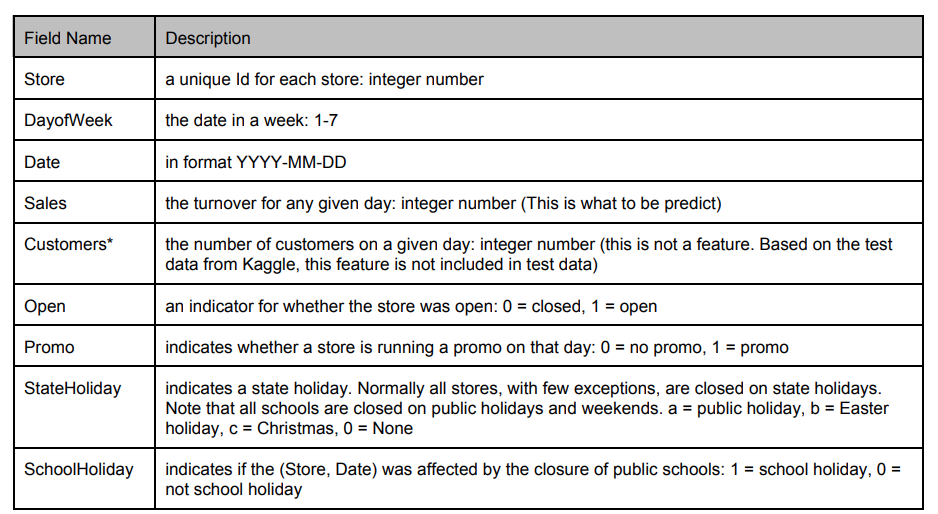
\includegraphics[width=12cm]{image/t1.png}
        \caption{Historical sales data table features}
    \end{figure}


The second part of training data is supplement store information. It has 1115 store info entries, which listed
the store type, competitor and a different kind promotion info. Table 2 below describes all the field in this file.

\begin{figure}[H]
        \centering
       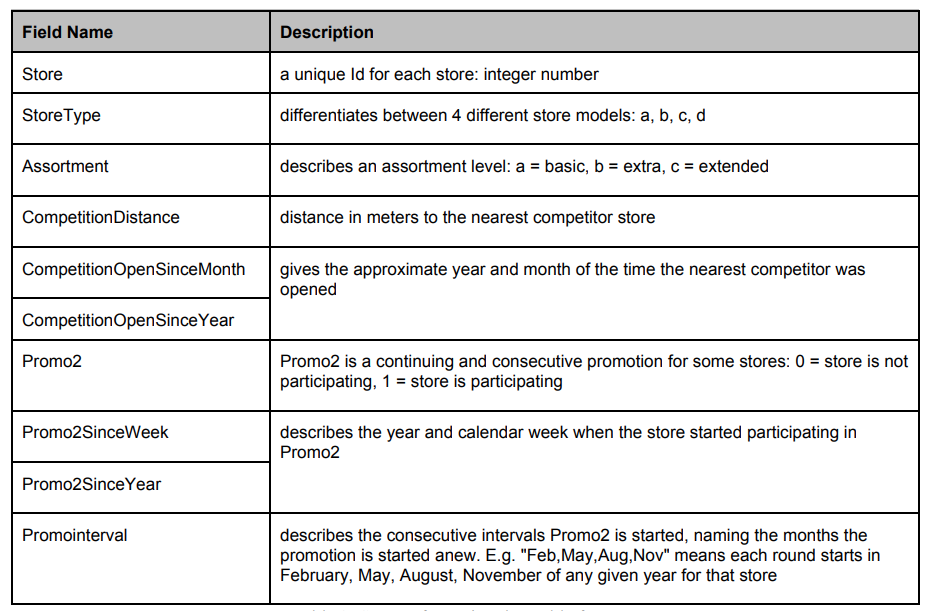
\includegraphics[width=12cm]{image/t2.png}
        \caption{Store Information data table features}
\end{figure}



Here the distribution of Sales

\begin{figure}[h]
\centering
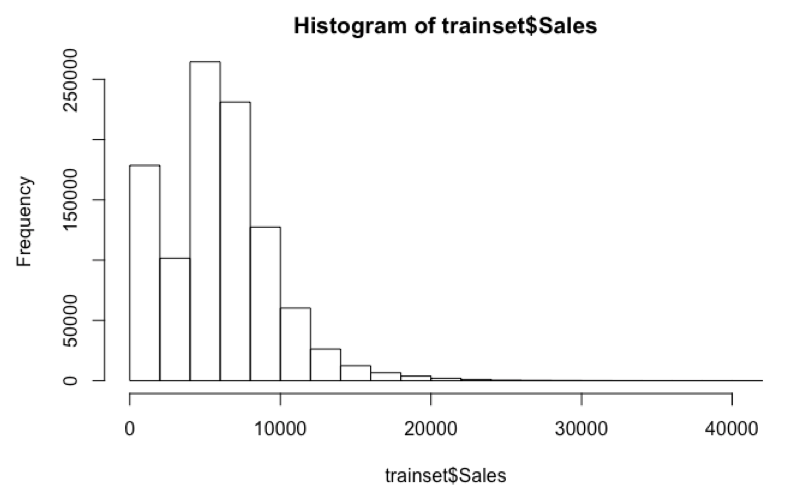
\includegraphics[width=10cm]{image/hist_sales.png}
\caption{hist of sales}
\label{fig3}
\end{figure}


We have previously speculated that the store id has a relationship with sales. It is possible that the smaller the store id is, the it was built early, so it is more likely to be in the city center, so the sales are higher.But from the graph we can see that sales are not related to store id.
\begin{figure}[h]
\centering
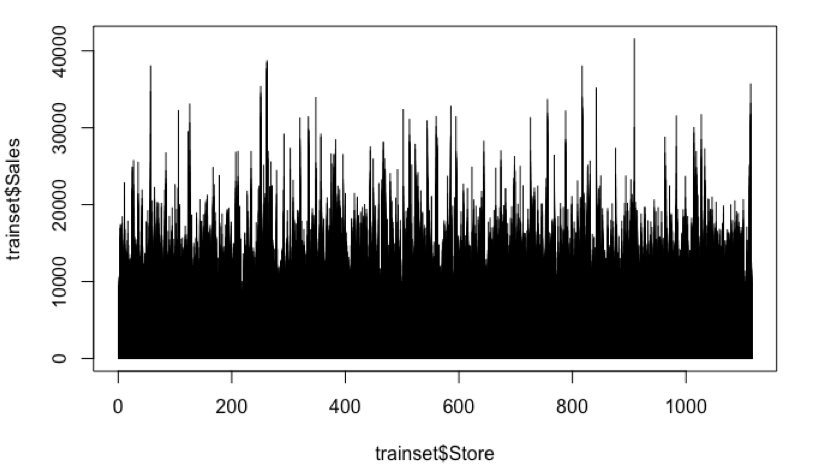
\includegraphics[width=10cm]{image/relationship_between_store_id_and_sales.png}
\caption{relationship between store id and sales}
\label{fig4}
\end{figure}




We can see that most stores are closed on Sundays, while sales are more higher on Monday.

\begin{figure}[h]
\centering
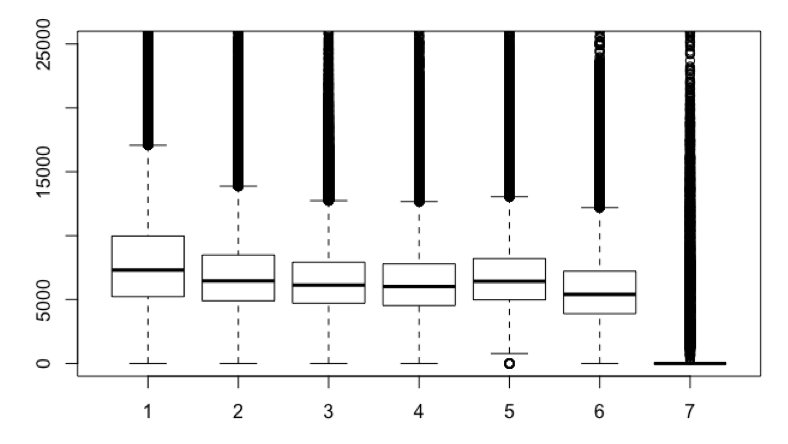
\includegraphics[width=10cm]{image/relationship_between_day_of_week_and_sales.png}
\caption{relationship between day of week and sales}
\label{fig5}

\end{figure}



\newpage
It can be seen that each year from October to December  is a period of rapid growth, December to the peak, and from January to the bottom. And the overall fluctuations are also obvious.

\begin{figure}[h]
\centering
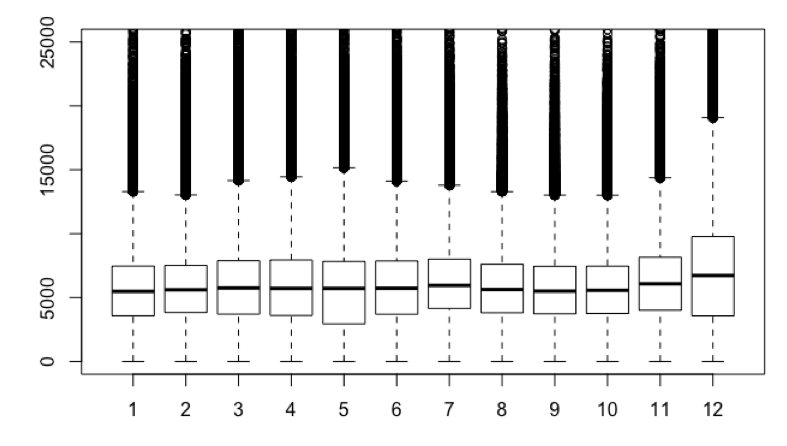
\includegraphics[width=10cm]{image/relationship_between_month_and_sales.png}
\caption{relationship between month and sales}
\label{fig6}
\end{figure}



\begin{figure}[h]
\centering
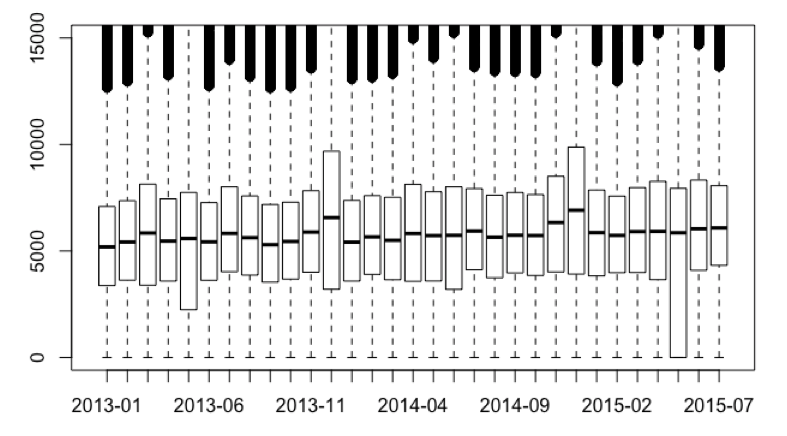
\includegraphics[width=10cm]{image/relationship_between_year_month_and_sales.png}
\caption{relationship between year and month and sales}
\label{fig7}
\end{figure}




\newpage 
It can be seen that in a certain distance range, many stores will get higher sales than other stores.
\begin{figure}

\centering
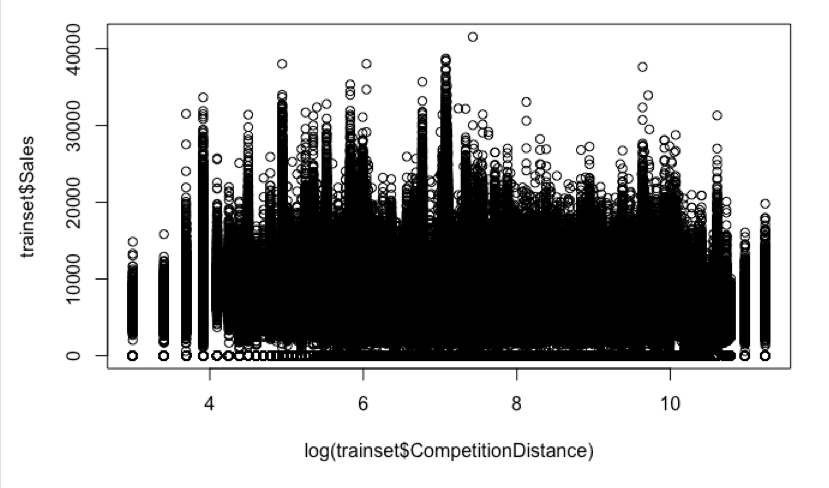
\includegraphics[width=10cm]{image/relationship_between_day_of_competition_distance_and_sales.png}
\caption{relationship between competition distance and sales}
\label{fig8}
\end{figure}


The same day sales are obviously better than non-promotional sales, but the difference is not very big.

\begin{figure}[h]
\centering
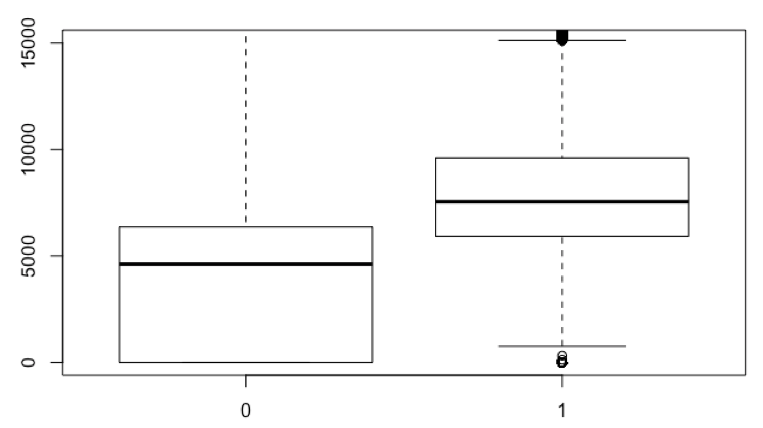
\includegraphics[width=10cm]{image/relationship_of_having_promo_or_not.png}
\caption{relationship of having promo or not}
\label{fig9}
\end{figure}


\newpage
The first state holiday has more effect on sales than the others.

\begin{figure}[h]
\centering
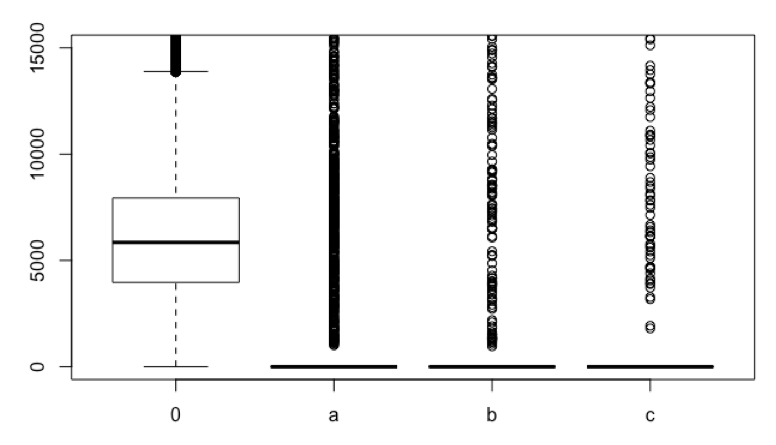
\includegraphics[width=10cm]{image/relationship_of_having_stateholiday_or_not.png}
\caption{relationship of having stateholida or not}
\label{fig10}
\end{figure}



The school holiday has little effect on sales.


\begin{figure}[h]
\centering
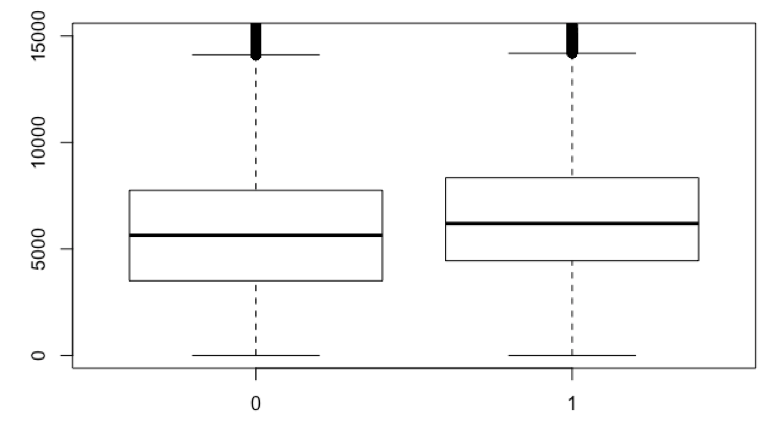
\includegraphics[width=10cm]{image/relationship_of_having_schoolholiday_or_not.png}
\caption{relationship of having schoolholida or not}
\label{fig10}
\end{figure}


\newpage
For StoreType, it can be seen that b type sales are higher than others, and there is basically no difference between a, c, and d types.

\begin{figure}[h]
\centering
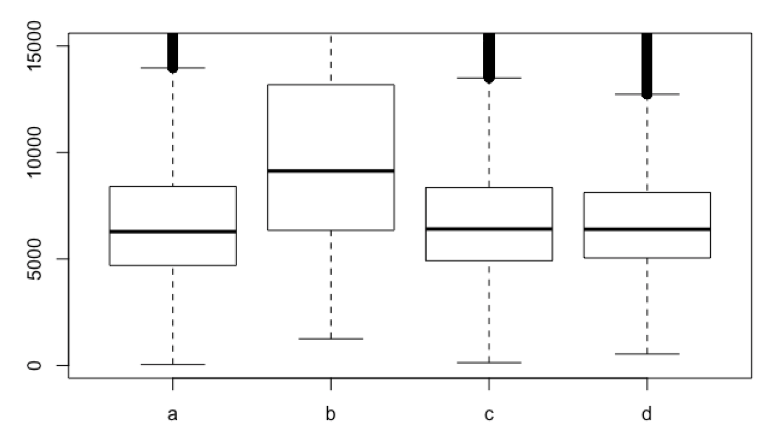
\includegraphics[width=10cm]{image/relationship_of_storetype.png}
\caption{relationship of storetype}
\label{fig11}
\end{figure}


Sales without a promotion type 2 are overall better.So it can be seen that the promotion2 has little effect on the customer.

\begin{figure}[h]
\centering
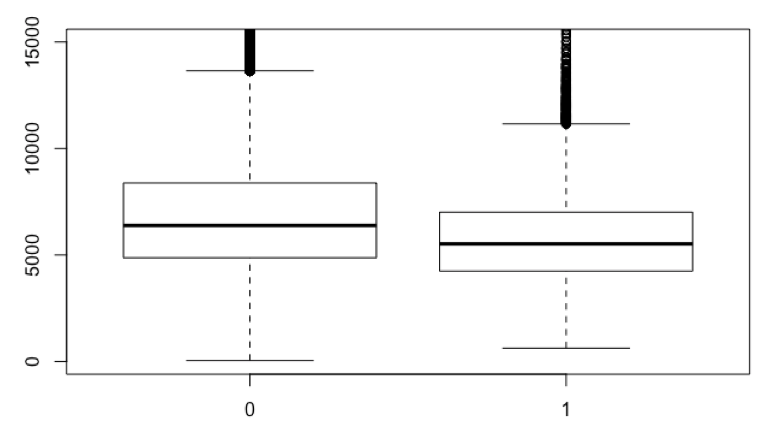
\includegraphics[width=10cm]{image/relationship_of_having_promo2_or_not.png}
\caption{relationship of having promo2 or not}
\label{fig13}
\end{figure}

\newpage
\section {Data processing}
\subsection{CompetitionDistance}
CompetitionDistance is a feature of store table , when we merge train store and store table , this feature will give us the wrong information . For exemple , the CompetitionDistance of store 1 is 1000, CompetitionOpenSinceYear and CompetitionOpenSinceMonth tell us the moment where his competator opened. So, we cannot say that CompetitionDistance is also 100O in the day before this moment , beacause this store even dont have a competator before this moment.

So,we compared the date and competitor open date. For any date and any store which doesn’t has competitor in this date, we assign CompetitionDistance as a large number 100000.

\subsection{Promo2}
Similarly, we treated Promo2 for the same reason, but it is more complicated .Because we also take PromoInterval into account. So, we combined Promo2, Promo2SinceWeek, Promo2SinceYear and Promointerval to a promotion 2
indicator in historical sales data. The indicator indicates on a certain day whether a certain store is on promotion 2.

\subsection{Store and Sales}
We treated Store as a factor and we did a log transform for sales in oder to not be so sensitive to high sales.

\section{\textbf{Methodology}}

\subsection{Linear Model}

For this problem, the linear models have bad performances, but there are also a way to build a linear model. Here we tried `linear regression' , `Ridge Regression' and ` Lasso Regression'. To make some features working such as `DayOfWeek', `StoreType' and `Assortment', we use the ont hot function from package `mltools'. As the results,  all of these three regression have a test error feedbacked from kaggle.com which is arroud 0.4. 

\subsection{\textbf{SVM}}

	For the SVM method, we choose the package ``e1071" to train our model, so our first step is choosing the regression type and the kernel for this regression. 

	\subsubsection{Kernels and Type selection:}

	\begin{center}
	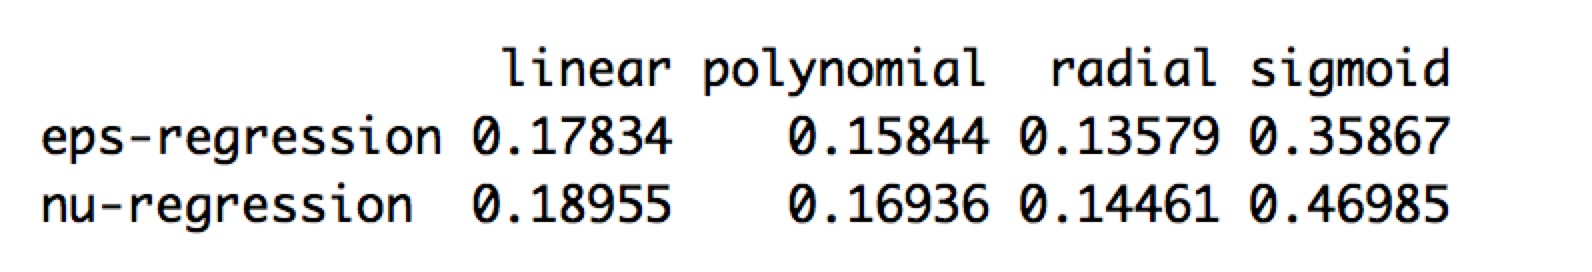
\includegraphics[width=5in]{image/svmkernal.png}\\
	FigureX: Train Error with different kernels and types used in SVM regression
	\end{center}

	We can see that with the Kernel `radial' and the type `eps-regression', the model permance better.

	\subsubsection{Parameter Choosing:}

	Here we use the function `tune.svm' from the package ``e1071" to compare the different gamma and cost. This function use K-ford cross validation to choose the parameter. The gamma parameter defines how far the influence of a single training example reaches. The cost parameter rules the error of the cutting plane. With higher cost the train error will be lower but the test error may growth, and the parameter gamma is for the Kernel, it's also sensitive for our model.

	\begin{center}
	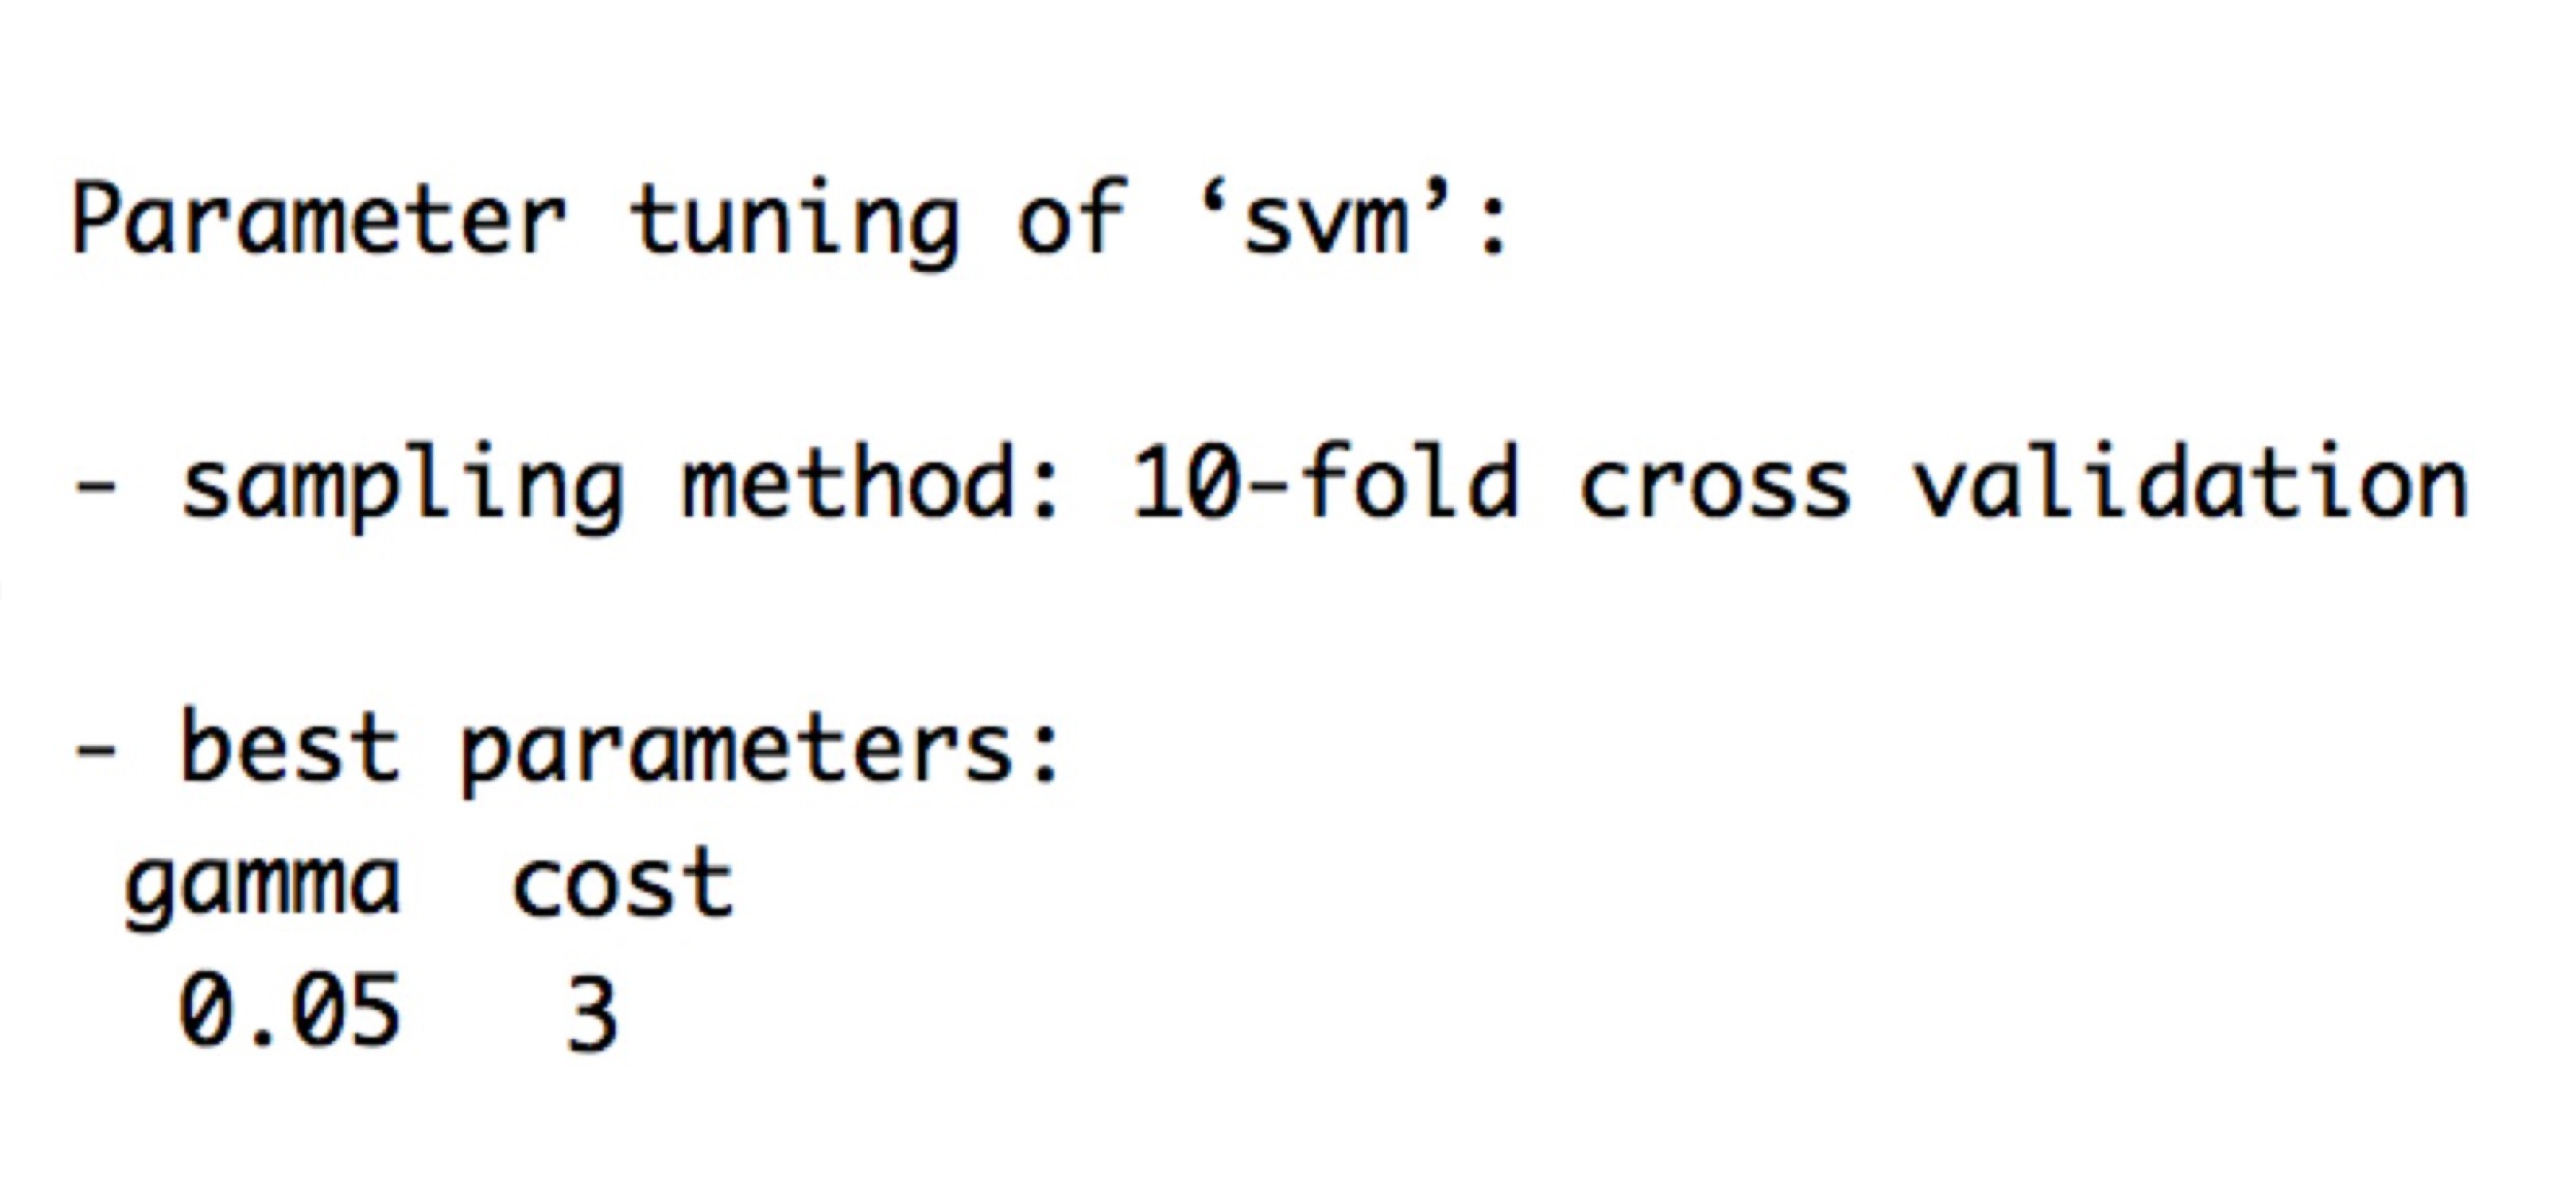
\includegraphics[width=5in]{image/svmp.jpeg}\\
	FigureX: Best Parameter
	\end{center}

	\subsubsection{Result:}

	Because of the running time of the svm model is long, we didn't pay too much attention into this model. Our result error is .

	\begin{center}
	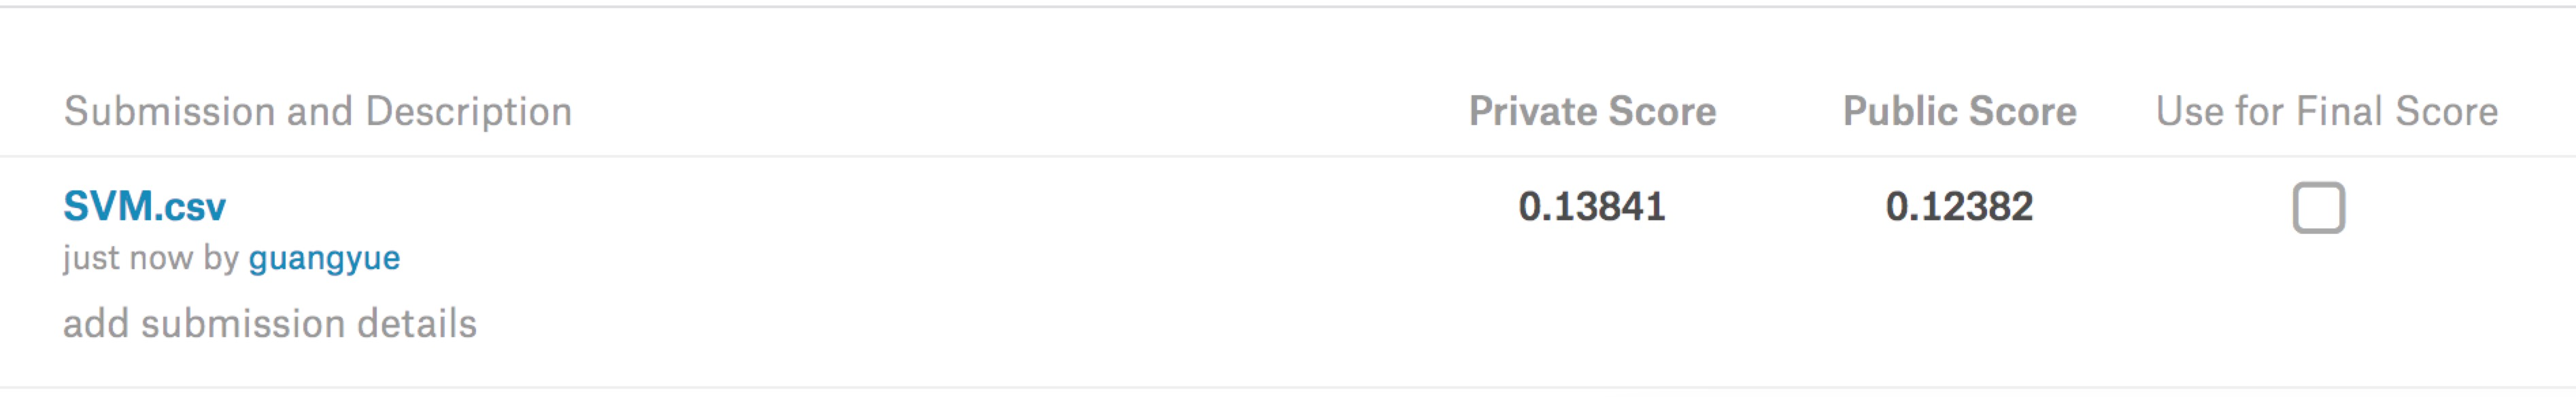
\includegraphics[width=9in]{image/svmres.png}\\
	FigureX: Result
	\end{center}

\subsection{Random Forest and H2o}

	\subsubsection{Random Forest:}
	
	Random Forest is a flexible, `easy to use' machine learning algorithm, it porduce a good result most of the time. It is also one of the most used algorithms, because it's simplicity and the fact that it can be used for both classification and regression tasks.

	When given a set of data, Random Forest generates a forest of classification or regression trees, rather than a single classification or regression tree. Each of these trees is a weak learner built on a subset of rows and columns. It chose the features and the subset of the data(for training a tree) randomly. More trees will reduce the variance. So it could handle well the overfitting issues. For our problem, it has also a good performance.

	\subsubsection{H2o Random Forest:}

	`H2o' package use Distributed Random Forest, which is a powerful classification and regression tool. For this package, `h2o.randomforest' run faster than the normal one in R, it can also limit the tree depth, (R's randomForest builds really deep trees), allowing for having a better predictions.

	\subsubsection{Parameter Choosing:}

	So here we should choose the parameter `max\_depth', here we use Cross-Validation to compare the test error.

	\begin{center}
	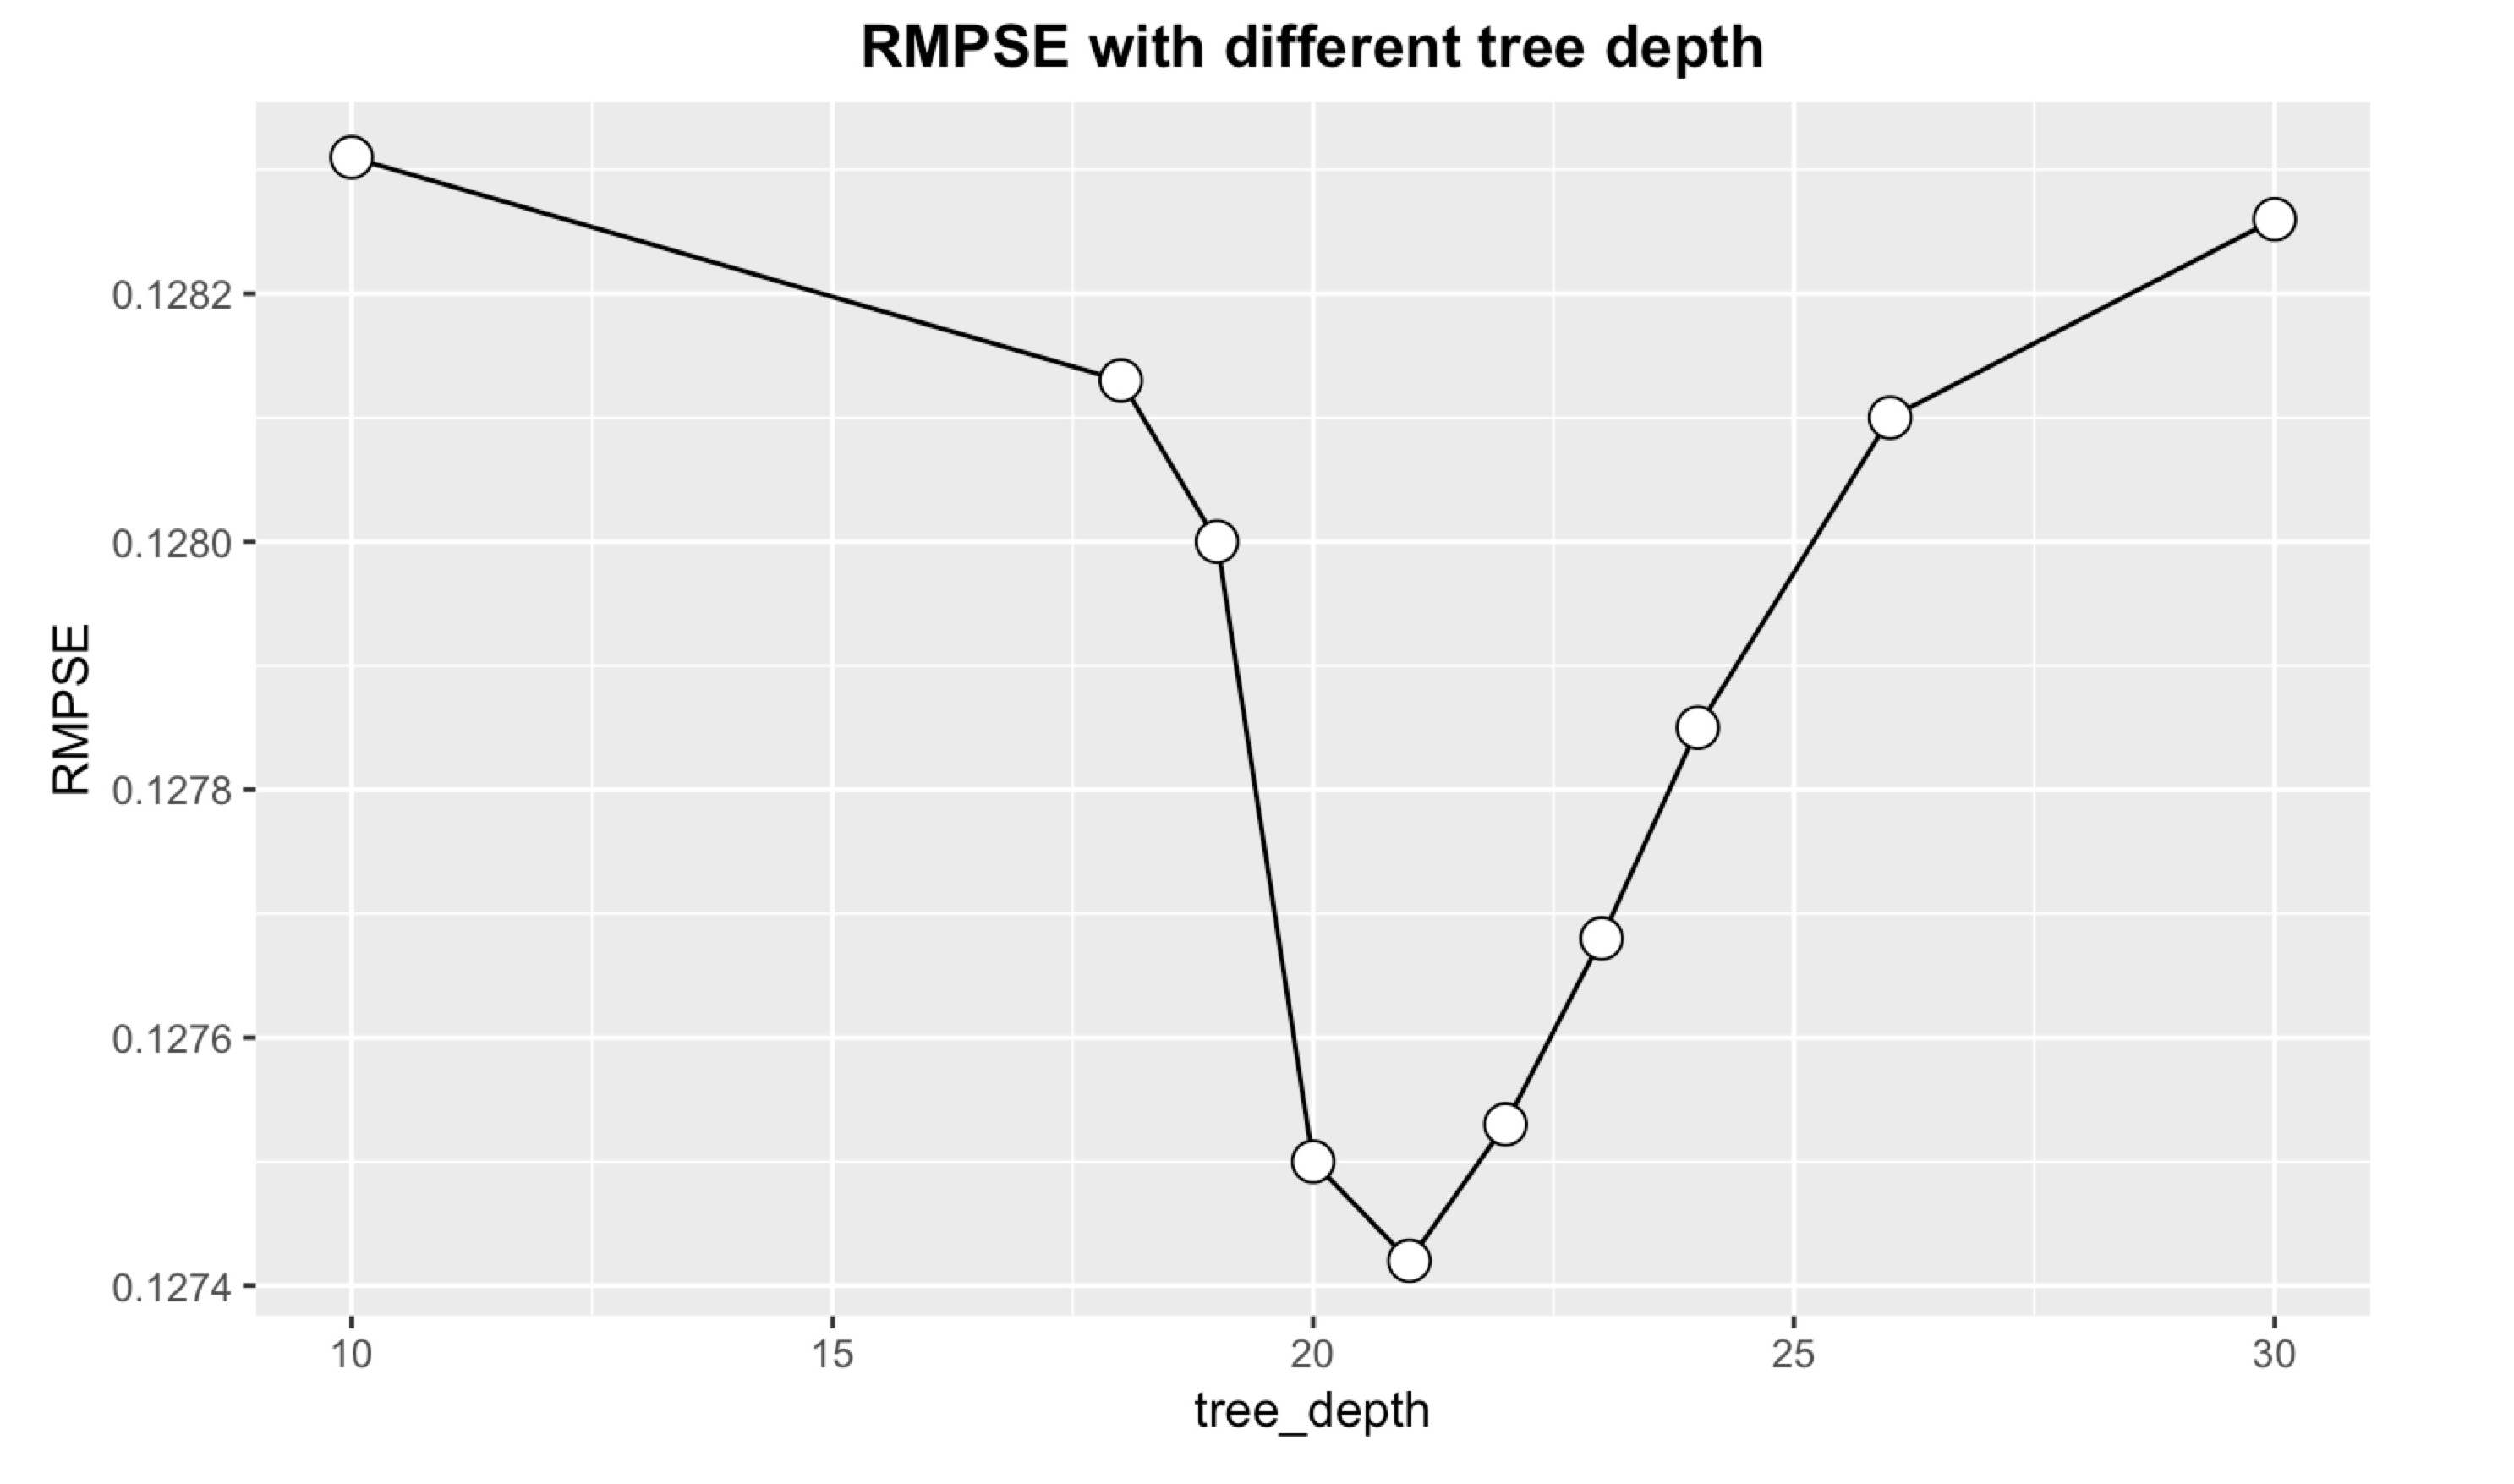
\includegraphics[width=5in]{image/cross.png}\\
	FigureX: RMPSE with different tree depth
	\end{center}

	We can see that for the test error, the models with depths 20 and 21 have the best porfermences. So we decided to build two models with the depth which are 21 and 20. Then we build a forest with a big quantity of trees, Which is 100.

	\subsubsection{Feature Selection:}

	For h2o random forest, we should load the data into h2o cluster. After our several test, we find that some features make the models perform worse. With the summary of our model, we decide to remove some features which have a low importance to our model. After we remove two features `SchoolHoliday' and `StateHoliday', our random forest model perform better.

	\subsubsection{Result:}

	\begin{center}
	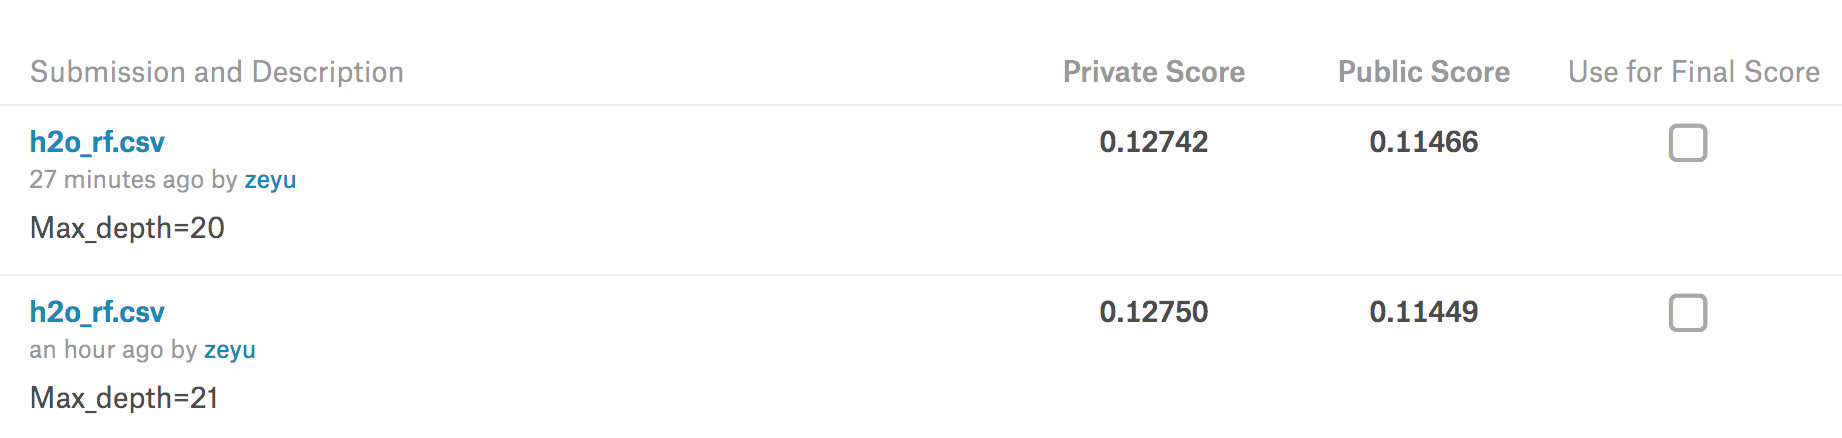
\includegraphics[width=9in]{image/h2ores.png}\\
	FigureX: The Result Of Our Models
	\end{center}	

	We run our best models on kaggle.com provided test data. The test errors feedbacked	from kaggle.com are 0.11449 and 0.11466. So we can say that the forest with depth maximum 21 is better. And this result is already in the top 150 on kaggle.com. 
\newpage
\section{\textbf{Conclusion}}

According our results,  Random Forest has the lowest test error feedbacked from kaggle.com. But we believe that the SVM model could perform as well as RF although it cost so much time for learning once. So for our future work, we will do more anlyses and tries on SVM.

After this project, we realize that the feature treatment has a large impact on training model quality. A correct feature selection could helps us to develop simpler and faster models. Once features are chosen and formatted correctly, the prediction error improved dramatic. Data preprocessing is the same, because, the representation and quality of data is first and foremost before running an analysis. 

What's more, after this project, we have an unforgetable experience of data analysis. We know clearly the steps to treat the data and train the machine learing models, and have a clearer understanding of models such as Random Forest and Support Vector Machine.

\section{\textbf{Reference}}

1. Data source:\href{https://www.kaggle.com/c/rossmann-store-sales/data}{https://www.kaggle.com/c/rossmann-store-sales/data}

2. Distributed Random Forest Introduction:\href{http://docs.h2o.ai/h2o/latest-stable/h2o-docs/data-science/drf.html}{http://docs.h2o.ai/h2o}

3. Data preprocessing and feature selection:(en chinois)\href{https://blog.csdn.net/u010089444/article/details/70053104}{https://blog.csdn.net}

4. Support Vector Machine: \href{http://uc-r.github.io/svm}{http://uc-r.github.io/svm}

\end{document}
